\PassOptionsToPackage{usenames,dvipsnames}{xcolor}

\documentclass[20pt, a0paper, landscape, margin=0mm, innermargin=15mm, blockverticalspace=15mm, colspace=15mm, subcolspace=8mm]{tikzposter}
\usepackage[T1]{fontenc}
\usepackage[utf8]{inputenc}
\usepackage[english]{babel}

\usepackage{amsmath,amsfonts,amssymb,mathtools}

%\usepackage[usenames,dvipsnames]{xcolor}
\usepackage{graphicx,mwe}
\usepackage{filecontents}% http://ctan.org/pkg/filecontents
\usepackage{tikz}
\usepackage{multicol}
\usepackage{adjustbox}
\usepackage{authblk}

\usepackage{enumitem}

\usepackage{caption}
\captionsetup{font=large}

\usepackage{url}
\usepackage[colorlinks=false]{hyperref}
\urlstyle{tt}


%\newcommand*{\doi}[1]{\href{https://doi.org/#1}{\nolinkurl{https://doi.org/#1}}}
\newcommand*{\doi}[1]{\href{https://doi.org/#1}{\nolinkurl{doi:#1}}}


% university colors based on branding guides
\definecolor{OSUorange}{HTML}{C34500}
\definecolor{UConnBlue}{HTML}{000E2F}
\definecolor{GoogleBlue}{HTML}{0266C8}

% \makeatletter
% \def\TP@titlegraphictotitledistance{-4cm}
% \settitle{ \centering \vbox{
% \@titlegraphic \\ [\TP@titlegraphictotitledistance] 
% \centering
% \color{titlefgcolor} {\bfseries \Huge \@title \par} % add \sc for smallcaps
% \vspace*{2em}
% {\huge \@author \par} \vspace*{1em} {\LARGE \@institute}
% }}
% \makeatother

%% Code for increasing tikzfigure caption font size
% \renewenvironment{tikzfigure}[1][]{
%   \def \rememberparameter{#1}
%   \vspace{10pt}
%   \refstepcounter{figurecounter}
%   \centering
%   }{
%     \ifx\rememberparameter\@empty
%     \else %nothing
%     \\[10pt]
%     {\large Fig.~\thefigurecounter: \rememberparameter}
%     \fi
% }


%% Set up a logo on each side
\makeatletter
\newcommand\insertlogoi[2][]{\def\@insertlogoi{\includegraphics[#1]{#2}}}
\newcommand\insertlogoii[2][]{\def\@insertlogoii{\includegraphics[#1]{#2}}}
\newlength\LogoSep
\setlength\LogoSep{-8cm}

\insertlogoi[width=18cm]{OSU-color-horz}
\insertlogoii[width=10cm]{NRG-logo}

\def\TP@titlegraphictotitledistance{-4cm}
\settitle{ \centering \vbox{
%\@titlegraphic \\ [\TP@titlegraphictotitledistance] 
\centering
\color{titlefgcolor} {\bfseries \Huge \@title \par} % add \sc for smallcaps
\vspace*{2em}
{\huge \@author \par} \vspace*{1em} {\LARGE \@institute}
}}

\renewcommand\maketitle[1][]{  % #1 keys
    \normalsize
    \setkeys{title}{#1}
    % Title dummy to get title height
    \node[transparent,inner sep=\TP@titleinnersep, line width=\TP@titlelinewidth, anchor=north, minimum width=\TP@visibletextwidth-2\TP@titleinnersep]
        (TP@title) at ($(0, 0.5\textheight-\TP@titletotopverticalspace)$) {\parbox{\TP@titlewidth-2\TP@titleinnersep}{\TP@maketitle}};
    \draw let \p1 = ($(TP@title.north)-(TP@title.south)$) in node {
        \setlength{\TP@titleheight}{\y1}
        \setlength{\titleheight}{\y1}
        \global\TP@titleheight=\TP@titleheight
        \global\titleheight=\titleheight
    };

    % Compute title position
    \setlength{\titleposleft}{-0.5\titlewidth}
    \setlength{\titleposright}{\titleposleft+\titlewidth}
    \setlength{\titlepostop}{0.5\textheight-\TP@titletotopverticalspace}
    \setlength{\titleposbottom}{\titlepostop-\titleheight}

    % Title style (background)
    \TP@titlestyle

    % Title node
    \node[inner sep=\TP@titleinnersep, line width=\TP@titlelinewidth, anchor=north, minimum width=\TP@visibletextwidth-2\TP@titleinnersep]
        at (0,0.5\textheight-\TP@titletotopverticalspace)
        (title)
        {\parbox{\TP@titlewidth-2\TP@titleinnersep}{\TP@maketitle}};

    \node[inner sep=0pt,anchor=west] 
      at ([xshift=-\LogoSep]title.west)
      {\@insertlogoi};

    \node[inner sep=0pt,anchor=east] 
      at ([xshift=\LogoSep]title.east)
      {\@insertlogoii};

    % Settings for blocks
    \normalsize
    \setlength{\TP@blocktop}{\titleposbottom-\TP@titletoblockverticalspace}
}
\makeatother

\setlength{\columnsep}{2cm}


\title{\parbox{0.7\linewidth}{Swept rule domain decomposition for 1D PDEs on heterogeneous compute clusters}}

\author[1]{Daniel J.\ Magee}
%\institute{Oregon State University}
\author[2]{Kyle E.\ Niemeyer}

\affil[1, 2]{School of Mechanical, Industrial, and Manufacturing Engineering, Oregon State University}

\institute{\href{mailto:mageed@oregonstate.edu}{\nolinkurl{mageed@oregonstate.edu}} and \href{mailto:kyle.niemeyer@oregonstate.edu}{\nolinkurl{kyle.niemeyer@oregonstate.edu}}}

\date{}

\usetitlestyle{Filled}

\begin{document}

\maketitle

\begin{columns} % See Section 4.4
    \column{0.25} % See Section 4.4
    \block{Introduction \& Motivation}{
	Accurate, fast solutions to Partial Differential Equations are essential to simulating physical phenomena with ever increasing fidelity. This greater resolution provides insight that drives technological development, but requires extensive computational resources. Our project applies a new technique (the swept rule) for apportioning these resources (domain decomposition) in PDE solutions to heterogeneous computing clusters.
    \vspace{0.5em}
    
    Recently, high-performance computing clusters, such as ONRL's Titan, have moved hybrid processing paradigm by incorporating accelerating processors like GPUs. The features of GPU architecture originally designed for high resolution and frequency displays, hundreds to thousands of simple, parallel cores, a transparent memory hierarchy, and generous on-chip memory capacity, make it a natural tool for scientific computing.  
    \vspace{0.5em}
    
    \begin{minipage}{0.45\linewidth}
    \centering
    \begin{tikzfigure}
    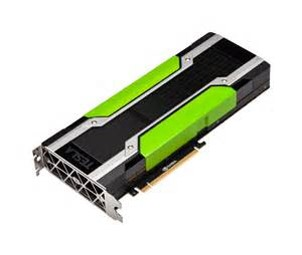
\includegraphics[width=\linewidth]{BigGpu}
    \end{tikzfigure}
    \captionof{figure}{GPU used in this study: Tesla K40c}
    \end{minipage}
    \hfill
    \begin{minipage}{0.45\linewidth}
    \centering
    \begin{tikzfigure}
    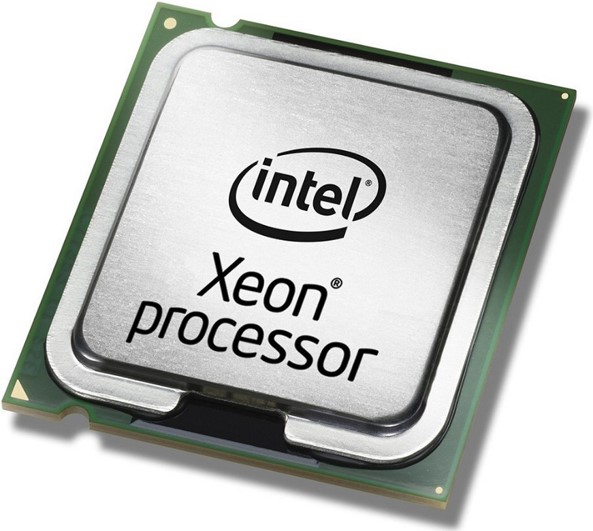
\includegraphics[width=\linewidth]{XEONCPU}
    \end{tikzfigure}
    \vspace{0.25em}
    \captionof{figure}{CPU used in this study: Intel Xeon 2630-E5}
    \end{minipage}
    
    \vspace{1.25em}
    
    }
    
    \column{0.5}
    \block{Performance results}{
    	
    \begin{minipage}{0.48\linewidth}
    \centering
    \begin{tikzfigure}
    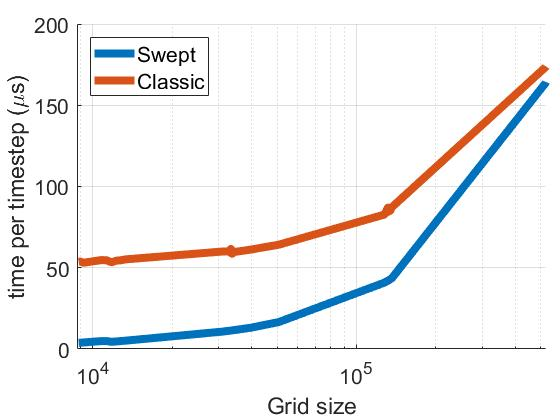
\includegraphics[width=\linewidth]{InitialCmpare}
    \end{tikzfigure}
    \captionof{figure}{Best execution times per timestep for the heat equation using swept and classic decompisition}
    \label{fig:rw}
    \end{minipage}
	\hfill
	\begin{minipage}{0.48\linewidth}
	\centering
	\vspace{0.25em}
	\begin{tikzfigure}
	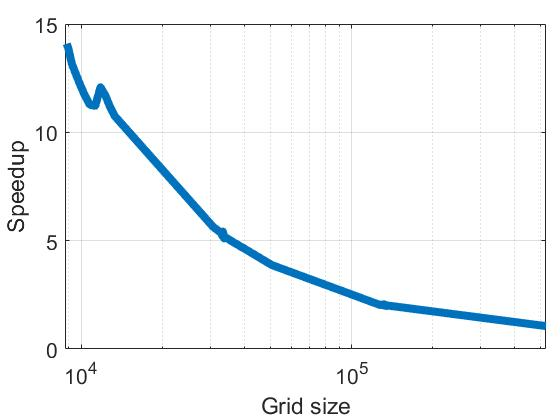
\includegraphics[width=\linewidth]{InitialSpeedup}
	\end{tikzfigure}
	\captionof{figure}{Speedup, $t_c/t_s$, of swept rule compared to classic decomposition.}
	\label{fig:sped}
	\end{minipage}
	
    \vspace{1em}
    
    These results are taken from an experiment which varies the node width, GPU affinity (the ratio of the grid partition size on the GPU to a single CPU process), and total grid size using $8$ MPI processes, one for each CPU core, one of which controls and communicates with the GPU. Figures~\ref{fig:rw} and~\ref{fig:sped} above compare the best times for the respective procedures at each grid size. 
    
    \vspace{1.75em}
    
    }
    
    \column{0.25}
    \block{Conclusions}{
	The results of this MPI+CUDA (GPU+CPU) implementation match previously observed trends in the GPU only implementation of the swept rule applied to the Heat equation:
	
	\vspace{0.75 em}
	
	\begin{itemize}
	 \item The performance benefits of the swept rule diminish with increasing grid size. As the cost of communication and kernel launch, which occur every sub-timestep in classic decomposition, become less significant as more computation is performed, the positive effect of the swept rule diminishes.
	 
	 \item The heat equation benefits from swept rule decomposition. This is because it permits a simple numerical scheme without path divergence that requires little memory overhead. Exploring more complicated equations that performed worse in the previous study, such as the Euler equations for inviscid flow, will provide a more general picture of performance benefit.
	 
	 \item The node width has a noticeable but minor impact on the performance of the swept rule.  In general node widths of $64 - 512$ produce the best results.  Additionally, GPU affinity did not substantially affect the results.
		
	\end{itemize}
	
	\vspace{0.75 em}
	
	These results are limited by the environment where they were obtained, a workstation with one CPU and one GPU. Distributed, heterogeneous environments incur substantially greater communication costs and diminish computation load per processor which should bolster the swept rule's comparative efficacy.
	
	\vspace{0.75em}
	
    }
\end{columns}

% bottom 
\begin{columns}
    \column{0.5}
    \block{Method}{
    \begin{minipage}[t]{0.3\linewidth}
	\centering\textbf{Classic Decomposition}   
    \begin{tikzfigure}
    \centering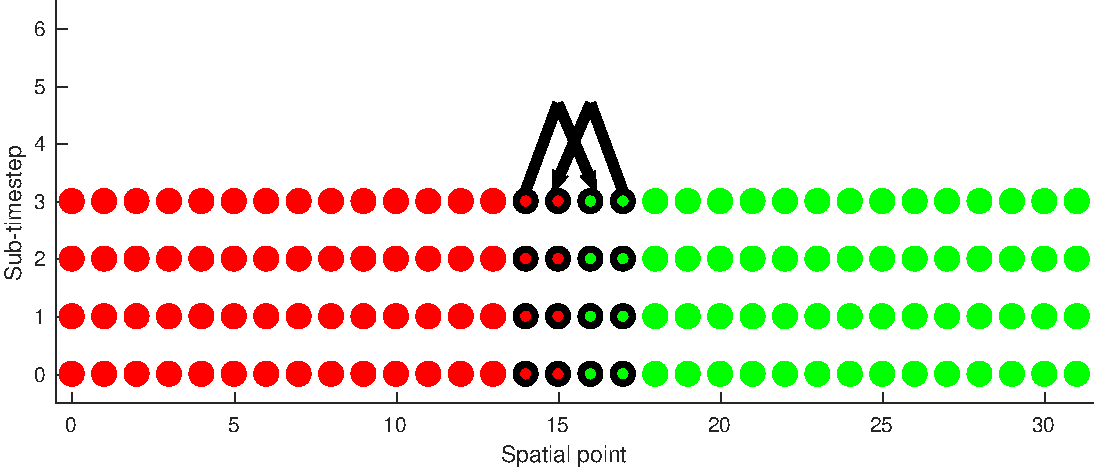
\includegraphics[width=0.86\linewidth]{ClassicScheme}
    \end{tikzfigure}
    \centering\textbf{Swept Decomposition}
    \begin{tikzfigure}
    \centering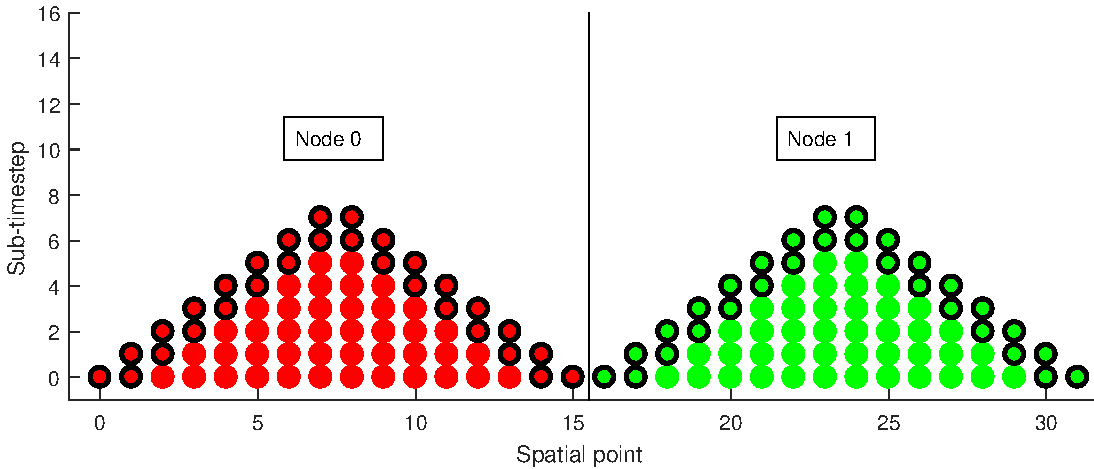
\includegraphics[width=0.88\linewidth]{FirstOrderStepOne}
    \end{tikzfigure}
    \begin{tikzfigure}
    \centering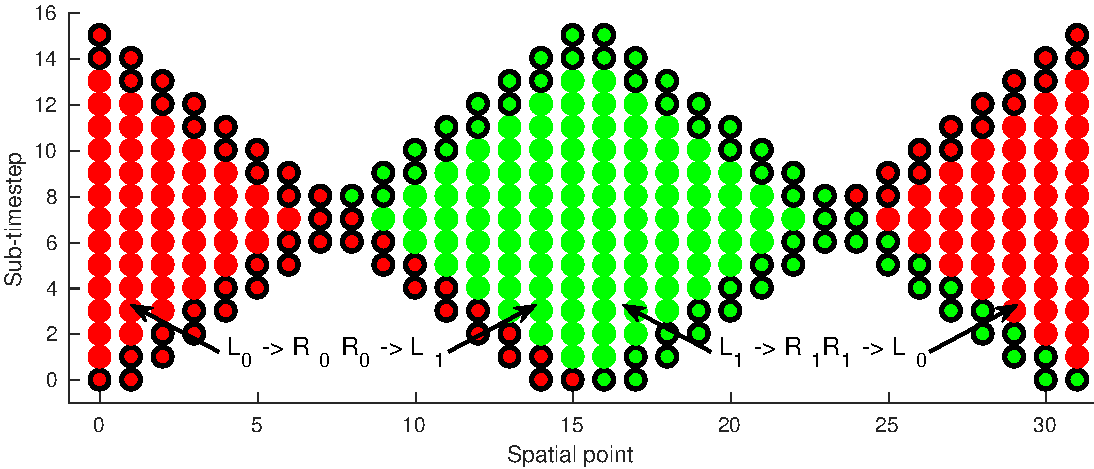
\includegraphics[width=0.88\linewidth]{FirstOrderStepTwo}
    \end{tikzfigure}
	\end{minipage}  
	\hfill
	\begin{minipage}[t]{0.69\linewidth} 
	As compute clusters become larger, more processors need to communicate to exchange results to continue a solution. The obvious answer to this challenge is to simply partition the spatial domain and pass the values at the edge of each node (partition) to the neighboring node. We refer to this decomposition method as Classic. 
	
	\vspace{0.75em}
	
	Since each sub-timestep, a step in a numerical method using a three-point spatial stencil, is dependent on the results of a previous sub-timestep, each process in a classic decomposition needs to communicate values at each edge spatial point to its neighbors after each sub-timestep. While the amount of data transferred in each communication is small, the latency cost of each communication event ($100\mu s - .5\mu s$) becomes significant over the many millions of timesteps needed to evaluate a meaningful equation with stability and precision.
	
	\vspace{0.75em}
	
	The swept rule seeks to mitigate this cost by exploiting the domain of dependence. As shown in the figures to the left, the swept rule marches forward in time computing all grid points for which all the dependent values are known. When there are no grid points with known stencils, it passes the values needed to continue to a neighboring node. In this way, it communicates twice while advancing across a number of sub-timesteps equal to the node width.
	
	\vspace{0.75em}
	
	The test case for the performance results presented here is the heat equation in one dimension, 
	\begin{equation}
	\frac{\partial T}{\partial t} = \alpha \frac{\partial^2 T}{\partial x^2} \;.
	\end{equation}

	Using a first-order, explicit, finite-difference approximation, forward differencing in time and central in space, we can solve for T at the new timestep,
	\begin{equation}
	T_i^{m+1} = \text{Fo} (T_{i+1}^m + T_{i-1}^m) + (1 - 2 \text{Fo}) T_i^m \;,
	\end{equation}
	where $i$ is the spatial node index and $m$ is the time index corresponding to time $t^m$.

	\end{minipage}
    }

    \column{0.25}
    \block{Works Cited}{
    \begin{enumerate}[leftmargin=1cm,topsep=0pt]
        
        \item DJ Magee \& KE Niemeyer. \texttt{HeterogeneousSwept1D}. GitHub: \url{https://github.com/Niemeyer-Research-Group/HeterogeneousSwept1D}.
        v1.0 (2017)
                 
        \item M Alhubail \& Q Wang.
        ``The Swept Rule for Breaking the Latency Barrier in Time Advancing PDEs.'' (2017) \textit{Journal of Computational Physics}, in press.
        \doi{10.1016/j.jcp.2015.11.026}
        
        \item DJ Magee \& KE Niemeyer.
        ``Accelerating solutions of PDEs with GPU-based swept time-space decomposition'' (2017) In preparation, available via {\tt \href{https://arxiv.org/abs/1705.03162}{arXiv:1705.03162}}.
		
    \end{enumerate}
    
    \vspace{1em}
    
    \textbf{Working Repository:}
    
   	\centering
\includegraphics[width=0.45\linewidth]{repoQR}

	\vspace{0.75em}

    }
   
    \column{0.25}
    \block{Acknowledgements}{
    This material is based upon work supported by NASA under award No.~NNX15AU66A under the technical monitoring of Drs.~Eric Nielsen and Mujeeb Malik.
    We also gratefully acknowledge the support of NVIDIA Corporation with the donation of the Tesla K40c GPU used for this research. 
    \\ \\
    \begin{minipage}{0.42\linewidth}
    \begin{tikzfigure}
    
\includegraphics[width=\linewidth]{cc-by}
    \end{tikzfigure}
    \end{minipage}
    \hfill
    \begin{minipage}{0.55\linewidth}
    This work is licensed under a Creative Commons Attribution 4.0 International License. To view a copy of this license, visit \url{http://creativecommons.org/licenses/by/4.0/}.
    \end{minipage}
    
    \vspace{2.5em}
%    \innerblock{Image credits}{
%    \small{
%    a: Modified from \url{https://www.olcf.ornl.gov/wp-content/uploads/2011/06/Oefelein2_web.png}, 
%    b: Weber et al., \emph{Combust Flame} (2014) \doi{10.1016/j.combustflame.2014.01.018}
%    c: Intel Skylake CPU \url{http://wimages.vr-zone.net/2015/04/Intel.jpg}
%    d: NVIDIA Tesla K40 \url{http://www.wiredzone.com/mmenglish/Images/actual}
%    e: Intel Xeon Phi \url{https://streamcomputing.eu/wp-content/uploads/2012/11/intel-xeon-phi-card.jpg}
%    }}
    
    \centering\textbf{Further Information}
    \vspace{0.5em}
    \colorlet{innerblocktitlebgcolor}{OSUorange}
    \colorlet{innerblocktitlefgcolor}{white}
    \innerblock{Niemeyer Research Group (OSU)}{\centering{\url{https://niemeyer-research-group.github.io}}}
    
    \vspace{2.5em}
    \colorlet{innerblocktitlebgcolor}{OSUorange}
    \colorlet{innerblocktitlefgcolor}{white}
    \innerblock{Daniel's Site }{\centering{\url{https://www.danieljmagee.com}}}
    
    \vspace{2.25em}
}
    
\end{columns}

\end{document}
